\documentclass[10pt]{beamer}
\usepackage{pgfpages}
%\usepackage[backend=biber,citestyle=verbose, bibstyle=apa]{biblatex}
\setbeameroption{show notes on second screen}
\usepackage[backend=biber, style=apa]{biblatex}
\addbibresource{main.bib}
\usetheme{metropolis}
%\addbibresource{demo.bib}
\usepackage{appendixnumberbeamer}
\usepackage{CJKutf8}
\usepackage{tipa}
\usepackage{amsmath}
\usepackage{xfrac}
\usepackage{bm}
\usepackage{suffix}
\usepackage{amssymb}
\usepackage{braket}
\usepackage{physics}
\usepackage{amsthm}
\usepackage{mathtools}
\usepackage{booktabs}
\usepackage{scalerel}
\usepackage[scale=2]{ccicons}
\usepackage{pgfplots}
\usepackage{subcaption}
\usepackage{algorithm}
\usepackage[noend]{algpseudocode} 
\usepackage{graphicx}
\usepackage{tikz}
\usepackage{mdframed}
\usepgfplotslibrary{dateplot}
%\let\footcite\footfullcite
\usepackage{xspace}
\usepackage{verbatim}
\newcommand{\themename}{\textbf{\textsc{metropolis}}\xspace}

\title{Pauli Path Integral Simulation}
\subtitle{For Noisy Variational Quantum Circuits}
\date{\today}
\author{Yuguo Shao}
\institute{Tsinghua University\\
Shanghai, ICCM 2024}
% \titlegraphic{\hfill\includegraphics[height=1.5cm]{logo.pdf}}

\begin{document}
\begin{CJK}{UTF8}{gbsn}
\maketitle
\note{Good morning, everyone. My name is Shao Yuguo, a Ph.D. student at Tsinghua University. 

It's a pleasure to be here today to introduce our recent work on the simulation of noisy variational quantum circuits.}

\begin{frame}{Table of contents}
  \setbeamertemplate{section in toc}[sections numbered]
  \tableofcontents[hideallsubsections]
\end{frame}
\note{In this talk, I will first introduce the background of quantum computing and the quantum supermacy in noisy intermediate-scale quantum (NISQ) era. 
  
 Then, I will discuss the potential of variational quantum algorithms, which are useful for solving practical problems and designed for NISQ devices.
  
 Finally, I will introduce our recent work on the simulation of noisy variational quantum circuits.
  
 Let's get started.}

\section{Introduction}
\begin{frame}[fragile]{Moore’s law}
  \begin{minipage}{0.23\textwidth}
    \begin{figure}
      \centering
      \includegraphics[width=\textwidth]{fig/moore0.png}
    \end{figure}
  \end{minipage}
  \begin{minipage}{0.75\textwidth}
    \vspace{3em}
    \begin{figure}
      \centering
      \includegraphics[width=\textwidth]{fig/moore1.png}
      \caption{Moore's Law. Source: \cite{quantum_computers}}
    \end{figure}
  \end{minipage}
  \begin{itemize}
    \item Moore's Law: The number of transistors on a microchip would double every two years, while the cost would be halved.
\end{itemize}
\end{frame}
\note{In 1965, Gordon Moore, the co-founder of Intel, predicted that the number of transistors on a microchip would double every two years, while the cost would be halved(halfed). 

This prediction has been proven(prove) to be true for the past 50 years. 

The figure shows the growth of the number of transistors from 1965 to 2015, shown in blue. 
The feature size which describes the size of the transistor, shown in yellow gets smaller and smaller.

}


\begin{frame}[fragile]{The End of Moore's Law \& Future of Computers}
  \begin{figure}
    \centering
    \includegraphics[width=0.8\textwidth]{fig/moore2.png}
  \end{figure}
  \begin{itemize}
    \item The feature size of the transistor is approaching the atomic scale.
    \item Quantum effects become significant.
    \item The development of new technologies is required.
  \end{itemize}
\end{frame}
\note{
  As the feature size of transistor approaches the atomic(a-tuo-mic) scale, Moore's law is facing challenges. 

In the atomic scale, the quantum effects become significant, and classical physics(phy-sic-s) is no longer valid.

This makes it impossible to continue the growth of the number of transistors on a microchip.

To continue the growth of computing power, the development of new technologies is required.

%Traditional silicon(ci-li-ken)-based computers are reaching their physical limits, and the development of new technologies is required to continue the growth of computing power. 

%Quantum computing is one of the most promising technologies that can potentially solve problems that are intractable(intra-ct-ble) for classical computers.
}


\begin{frame}[fragile]{Quantum Computing}
\begin{figure}
  \centering
  \begin{subfigure}[b]{0.2\textwidth}
    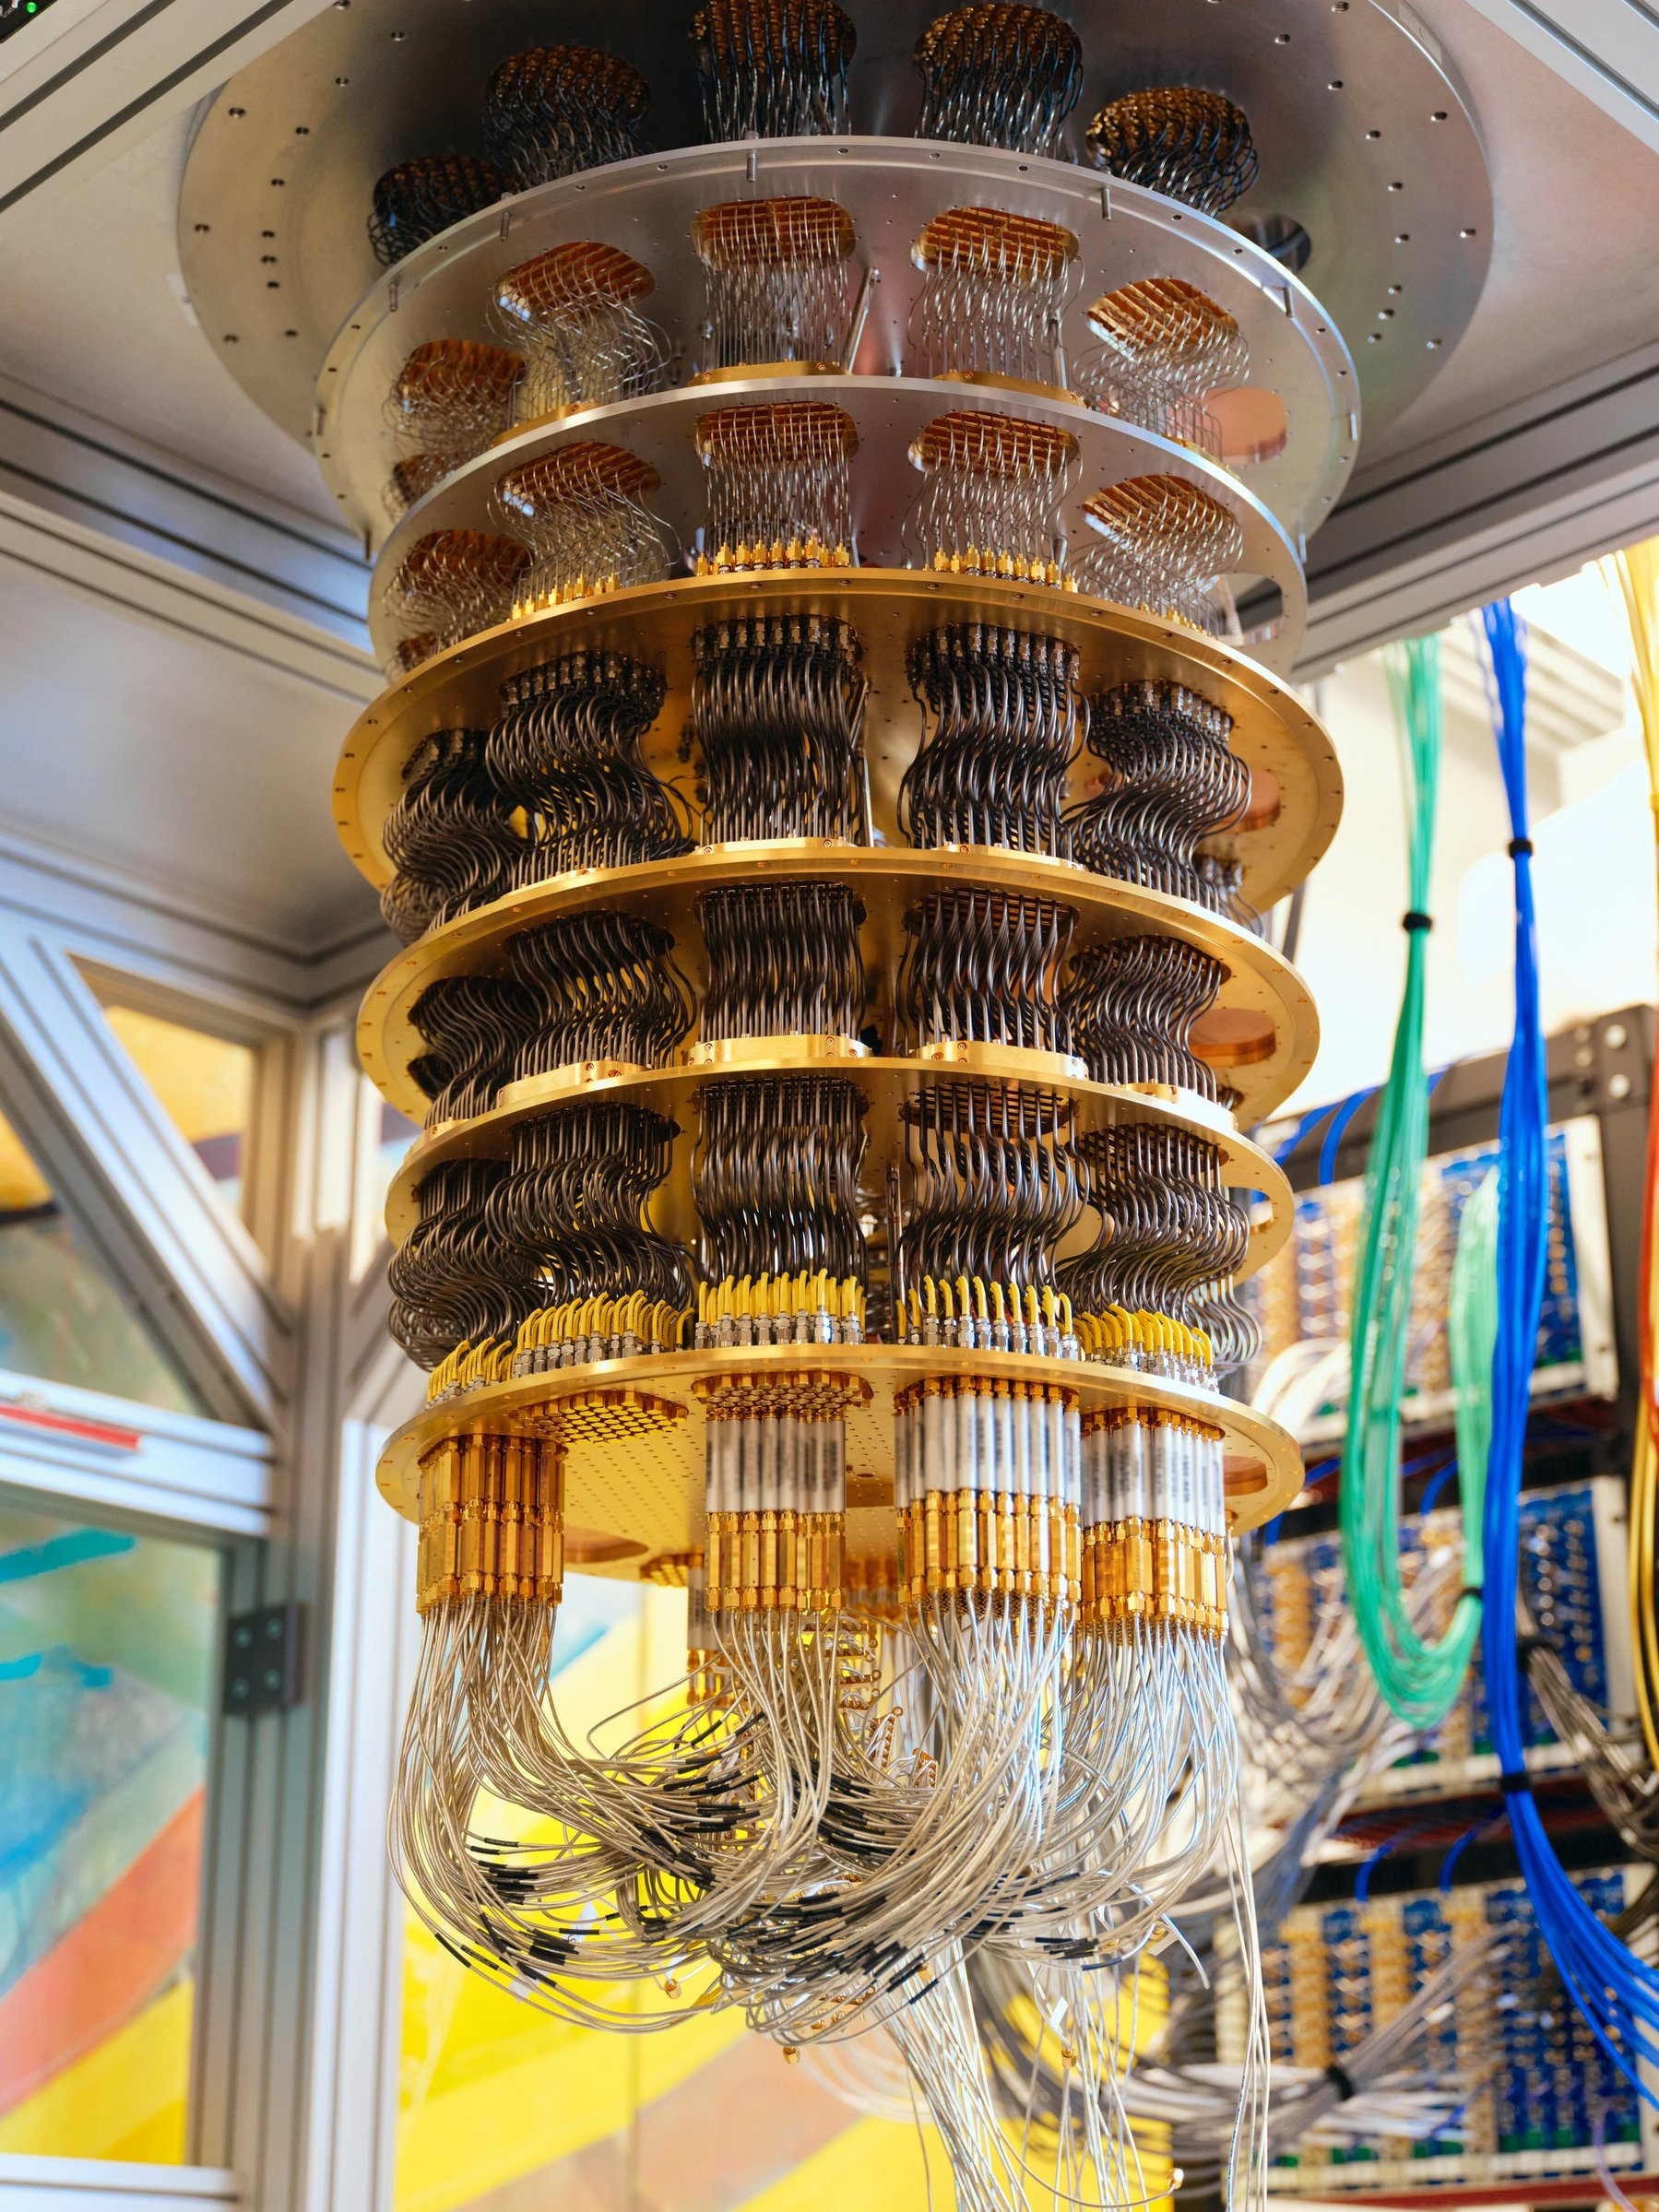
\includegraphics[width=\textwidth]{fig/google1.png}
  \end{subfigure}
  \hfill
  \begin{subfigure}[b]{0.3\textwidth}
    \includegraphics[width=\textwidth]{fig/newyorktimes.png}
  \end{subfigure}
  \hfill
  \begin{subfigure}[b]{0.4\textwidth}
    \includegraphics[width=\textwidth]{fig/chinatimes.png}
  \end{subfigure}
\end{figure}
\begin{itemize}
  \item Quantum Computing is a new paradigm of computation based on the principles of quantum mechanics.
  \item Google "Willow": 5 minutes vs 10,000,000,000,000,000,000,000,000 years (10 septillion years)
\end{itemize}
\end{frame}
\note{Recently, quantum computing has attracted(attract-ed) a lot of attention from both academia and industry(in-de-stry).

Compared to classical computers, quantum computers are based on the principles of quantum mechanics(mi-can-ni-kes), such as superposition and entanglement. 

These properties bring a new look to computing and have the potential to solve problems that are intractable(intra-ct-ble) for classical computers.

For example, last month Google announced their new quantum chip "Willow"(wei-low), which can solve a problem in 5 minutes that would take the world's fastest(fas-test) supercomputer in 10 septillion(sep-ti-lian) years.

%But what is quantum computing? And how does it work? Let's review the history of quantum computing.
}


\begin{frame}[fragile]{Historical Background}
  \begin{figure}
    \centering
    \includegraphics[width=0.3\textwidth]{fig/feynman.png}
  \end{figure}
  \begin{itemize}%~\footcite{feynman2018simulating}
    \item In 1982, Richard Feynman gave a talk at the first conference on quantum computation, entitled "Simulating Physics with Computers".
    \item When classical computers simulate quantum systems, the cost grows \textcolor{red}{exponentially} with the number of particles. 
    \item To build a computer based on quantum mechanics.
    %\begin{itemize}
    %    \item Quantum simulation: simulate quantum systems efficiently.
    %\end{itemize}
  \end{itemize}
\end{frame}
\note{It is generally believed that quantum computing was born() in 1982 when Richard Feynman proposed() the idea of creating a computer based on the laws of quantum mechanics.

Feynman pointed out that when classical computers simulate quantum systems, as the number of particles increases, the time required for calculation will increase exponentially. %which is completely incompetent(in-com-pe-tent). 

The solution is to build a computer based on quantum mechanics. 

%This motivation is called quantum simulation, which aims to simulate quantum systems efficiently. 

%And it remains one of the core purposes of building quantum computers today.
}


\begin{frame}[fragile]{Shor's Algorithms}
  \begin{itemize}
    \item In 1994~\footfullcite{shor1994algorithms}, Peter Shor proposed a quantum algorithm that can factorize large numbers in \textcolor{red}{polynomial time}.
    \item Large numbers factorization: Knowing big number $N$, which is the product of two prime numbers $p$ and $q$. What are $p$ and $q$?
    \begin{itemize}
      \item The best classical algorithm: \textcolor{red}{sub-exponential} time.
      \item The intractability of the factorization problem is the cornerstone of modern encryption, such as RSA.
    \end{itemize}
    \begin{figure}
      \centering
      \includegraphics[width=0.8\textwidth]{fig/shor.png}
    \end{figure}
    %\item In 1996~\footcite{grover1996fast}, Lov Grover proposed a quantum algorithm that can search an unsorted database in \textcolor{red}{quadratic time}, while the best classical algorithm is \textcolor{red}{linear}.
  \end{itemize}
\end{frame}
\note{In 1994, Peter Shor proposed a quantum algorithm that can factorize(fact-rize) large numbers in polynomial time.

The factorization of large numbers is a classic problem.% in number theory(see-ri). 
Given a big number N, which is the product of two prime(pri-me) numbers p and q. The  question is what p and q are?

The best classical algorithm for factorization is sub-exponential(ex-po-nential) time.

The intractability(intra-ct-a-bile-ty) of the factorization problem is the cornerstone(cor-ner-stone) of modern encryption(en-cre-pu-tion), such as RSA.

%And the quantum algorithm poses(po-ses) a threat(si-rea-te) to the security of many commercial encryption systems.

Here is a comparison(com-par-re-sen) between the classical and quantum algorithms for factorization.

It is estimated that a 4K-length RSA key can be broken in 4 hours by a quantum computer. While even for classical computers in 2042, it will take 10 to 22 years.}


\begin{frame}[fragile]{Quantum Error Correction}
  \begin{itemize}
    \item The quantum system inevitably interacts with the environment, leading to the loss of quantum information.
    \item These noises make the computation tasks impossible.
    \item Quantum error correction is a promising way to protect quantum information from noise.
    \begin{itemize}
      %\item Quantum error correction codes: encode quantum information in a larger Hilbert space.
      \item Quantum error correction is difficult due to the properties of quantum mechanics.
      \begin{itemize} 
      \item No-cloning theorem
      \item Collapse of the wave function
      
      \dots
      \end{itemize}
    \end{itemize}
  \end{itemize}
\end{frame}
\note{%Depending on complexity theory, quantum computers are believed to be able to solve certain problems exponentially faster than classical computers.

After the proposal of Shor's algorithm, the actual construction of quantum computers becomes a hot topic. Academia, industry, and even governments have invested a lot of resources in this field.

However, the development of quantum computers is not as smooth as expected(ex-pec-ted). 

The quantum information is easily destroyed by the environment, leading to a process(pro-cess) called decoherence.

This makes the computation tasks impossible.

To address this issue, quantum error correction is a promising way to protect quantum information.

However quantum error correction is difficult due(du-to) to the properties of quantum mechanics, such as the no-cloning(clone-lin) theorem(see-rem) and the collapse(co-la-pse) of the wave function.
}

\begin{frame}[fragile]{Error Correction is Expensive}
 The implementation of quantum error correction is described in seven stages, described in 2013. %Each advancement requires mastery of the preceding stages, but each also represents a continuing task that must be perfected in parallel with the others. Superconducting qubits are the only solid-state implementation at the third stage, and they now aim at reaching the fourth stage (green arrow). In the domain of atomic physics and quantum optics, the third stage had been previously attained by trapped ions and Rydberg atoms. No implementation has yet reached the fourth stage, where a logical qubit can be stored, via error correction, for a time substantially longer than the decoherence time of its physical qubit components.
  \begin{figure}
    \begin{tikzpicture}
      \node[anchor=south west,inner sep=0] (image) at (0,0) {\includegraphics[width=0.9\textwidth]{fig/339_1169_f1.jpeg}};
      \begin{scope}[x={(image.south east)},y={(image.north west)}]
        \draw[red,thick,<-] (0.8,0.85)--(0.85,0.9) node[anchor=south west] {Factoring Algorithm};
      \end{scope}
    \end{tikzpicture}
    \footcite{devoret2013superconducting}
  \end{figure}
  \begin{itemize}
    \item In 2024, Google ``Willow'' reached the fourth stage.
  \end{itemize}
\vspace{0.5em}
\end{frame}
\note{The implementation of quantum error correction is described in seven stages, as shown in the figure. 

%Each advancement requires mastery of the preceding stages, but each also represents a continuing task that must be perfected in parallel with the others.

In 2013, we were at the third stage and tried to reach the fourth stage, as the green arrow shows.

The third stage describes the necessary operations for quantum error correction such as measurement and control can be performed.

The fourth stage is the logical qubit has a longer coherence time than the physical qubits.

In other words, it describes the error correction scheme(si-game) can bring positive effects in the real quantum devices.

Actually after 11 years, last month, by Google Willow, the quantum error correction reaches the fourth stage.

While the Shor's factorization algorithm is at the top stage.
}



\begin{frame}[fragile]{Noisy Intermediate-Scale Quantum (NISQ) Computers}
 %Fault-tolerant quantum computers are still far from reality. 
 Nowadays Quantum devices have entered the NISQ era, with the potential to achieve quantum advantages.
  \begin{itemize}
    \item Number of qubits: 50-1000
    \item Imperfect \textcolor{red}{noisy} gates: fidelity 99.9\%-99.999\%
    \item Limited connectivity: \textcolor{red}{nearest-neighbor} (superconducting qubits)
  \end{itemize}
  \begin{figure}
    \centering
    \includegraphics[width=0.8\textwidth]{fig/2010-2020d.png}\footcite{nisq}
    %\caption{Source: \footcite{nisq}}
  \end{figure}
  \begin{itemize}
    \item To explore the potential of NISQ devices to achieve quantum advantages.
  \end{itemize}
  \vspace{0.25em}
\end{frame}
\note{%Fault-tolerant(fou-te-to-le-rant) quantum computers can perform quantum computation reliably(relai-a-bo-ly). But the fault-tolerant quantum computers are still far from reality(re-a-lity).

Nowadays, quantum devices have entered the NISQ era, which stands for the Noisy Intermediate-Scale Quantum era. It is characterized(\textipa{ˈkærəktəˌraizd}) by the following features:

It has hundreds qubits, typically between 50 to 1000.

The gates are imperfect, with probabilities to introduce errors. 

And the connectivity of the gates is limited. Not all qubits can interact with each other directly.

As the right figure shows. 

Around 2020, a new direction is emerging(\textipa{ɪˈmɜːdʒɪŋ}) to explore the potential of NISQ devices to achieve quantum advantages. Or called quantum supremacy.
}

\section{Supremacy in NISQ Era}

\begin{frame}[fragile]{Quantum Supremacy}
 In 2019~\footfullcite{arute2019quantum}, Google was the first to announce the realization of quantum supremacy.
  %The task is a demo of quantum advantage, regardless of its practical value.
  \begin{figure}
    \centering
    \begin{subfigure}[b]{0.45\textwidth}
      \includegraphics[width=\textwidth]{fig/supremacy1.png}
    \end{subfigure}
    \hfill
    \begin{subfigure}[b]{0.4\textwidth}
      \includegraphics[width=\textwidth]{fig/supremacy2.png}
    \end{subfigure}
  \end{figure}
  \begin{itemize}
    \item \textcolor{red}{Random circuit sampling}  tasks: 53 qubits, 20 cycles
    \item "Sycamore" quantum computer completed in \textcolor{red}{200 seconds}, and Google claims that it would take the world’s fastest supercomputer \textcolor{red}{10,000 years}.
  \end{itemize}
  \vspace{2em}
\end{frame}
\note{In 2019, Google was the first to announce the realization(real-lai-zation) of quantum supremacy. 
They demo a task called random circuit sampling, which aims to get samples from the output distribution of a random quantum circuit.

The quantum circuit consists(\textipa{kənˈsists}) of 53 qubits and 20 cycles.

Their quantum computer Sycamore(\textipa{ˈsee,kəmɔ:r}) did it in two hundreds seconds, and Google claimed that it would take the world’s fastest supercomputer ten thousand years.
}


\begin{frame}[fragile]{Imperfect Quantum Devices}
 The Google's device "Sycamore" is limited
  \begin{itemize}
    \item Noisy qubits with decoherence process.
    \item Imperfect gates with a probability of error.
    \item Locality of the gates is limited, with low entanglement entropy.
  \end{itemize}
  \begin{figure}
    \centering
    \begin{subfigure}[b]{0.4\textwidth}
      \includegraphics[width=\textwidth]{fig/google2.png}
    \end{subfigure}
    \hfill
    \begin{subfigure}[b]{0.4\textwidth}
      \includegraphics[width=\textwidth]{fig/google3.png}
    \end{subfigure}
  \end{figure}
\end{frame}
\note{
The Google's device "Sycamore" is a typical NISQ device.
As mentioned before, it is noisy, with qubits subject to a decoherence process, and gates are imperfect.

And the connectivity of the gates is limited, as the left figure shows.
The black crosses represent the qubits, and the blue lines represent the gates between the qubits.

The qubits can only interact with their nearest(near-st) neighbors(nei-bors), which causes the low entanglement entropy.

And the low entanglement entropy leads to the efficiency of the tensor network based simulation methods.
}

\begin{frame}[fragile]{Challenge of Classical Simulation}
 The supremacy assertion was challenged by tensor network based simulation methods:
  \begin{itemize}
    \item IBM~\footcite{pednault2019leveraging} claimed that the problem can be solved in \textcolor{red}{2.5 days} by the classical supercomputer Summit.
    \item Cotengra~\footcite{gray2021hyper} simulate an amplitude~\footnote{The number of samples in Google's experiment is about $10^{6}$.} in \textcolor{red}{3000 years} with one Quadro P2000 GPU.
    \item Alibaba~\footcite{huang2020classical} simulate 64 amplitudes in \textcolor{red}{267 days} with one V100 GPU.
    \item ITP CAS~\footcite{pan2021simulating} simulate $2^{21}$ amplitudes in \textcolor{red}{149 days} with one A100 GPU.
  \end{itemize}
\end{frame}
\note{
 Soon after Google's experiment, a lot of simulation results was proposed, which challenged the quantum supremacy.% assertion(a-sear-tion).

 They reduce the time from ten thousand years to a hundreds of days.

 IBM claimed that the problem could be solved in 2.5 days by the classical supercomputer Summit.

 Cotengra simulates an amplitude in 3000 years with one Quadro P2000 GPU. The total number of amplitude in Google's experiment is about 10 to 6.

 Alibaba simulates 64 amplitudes in 267 days with one V100 GPU.

 Institute of Theoretical Physics, Chinese Academy of Sciences simulates 2 to 21 amplitudes in 149 days with one A100 GPU.
}


\begin{frame}[fragile]{Challenge of Classical Simulation}
 In 2021, real-time classical simulation of Google's circuit in \textcolor{red}{304s with 42 million cores}. This achieved the same speed as the "Sycamore" quantum computer.
  \begin{figure}
    \centering
    \begin{subfigure}[b]{0.6\textwidth}
      \includegraphics[width=\textwidth]{fig/google4.png}
    \end{subfigure}
    \hfill
    \begin{subfigure}[b]{0.4\textwidth}
      \includegraphics[width=\textwidth]{fig/google5.png}
    \end{subfigure}
  \end{figure}
\end{frame}
\note{
 Finally, in 2021, a real-time classical simulation of Google's circuit was proposed, which achieved the same speed as the "Sycamore" quantum computer.

 The simulation was completed on TaiHu ZhiGuang supercomputer and won the Gordon Bell Prize.
}



\begin{frame}[fragile]{Noise Effect}
 How does noise affect the quantum advantage in random circuit sampling task?
  \begin{itemize}
    \item In 2022, Aharonov et al.~\footfullcite{aharonov2022polynomial} rigorously proved that when \textcolor{red}{noise} is widely present, the computational cost of simulating the random circuit sampling task is \textcolor{red}{polynomial size} in the regime of anti-concentration of the output distribution.
  \end{itemize}


 RCS has no utility. How about other quantum algorithms?
\end{frame}
\note{
 Except for the low entanglement induced by the limited connectivity, the noise is another factor that affects the quantum advantage in random circuit sampling task.

 In 2022, a work proposed a method to simulate the random circuit sampling task with noise. 
 They rigorously(\textipa{'rigərəsli}) proved that if the noise is widely present, the computational cost of simulating the random circuit sampling task is polynomial size in the regime of anti-concentration of the output distribution.

 The anti-concentration of the output distribution means that the output distribution is not concentrated on a few samples. When the random circuit is deep enough, the output distribution is anti-concentrated. It's a normal phenomenon in the random circuit sampling task.

 Another question is that the random circuit sampling task has no utility(u-ti-lety), it's a demo of quantum advantage. How about practical value quantum algorithms?

 Is it possible to achieve quantum advantage in NISQ devices with noise?
}

\section{Variational Quantum Algorithms}

\begin{frame}[fragile]{Variational Quantum Algorithms}
 Variational quantum algorithms are a class of quantum algorithms designed for NISQ devices. %, and are widely recognized as a potential pathway to achieve practical quantum advantages.
  \begin{figure}
    \centering
    \includegraphics[width=0.7\textwidth]{fig/vqa.png}\footcite{Cerezo2021variational}
  \end{figure}
  
  
 The basic idea is an analog of the deep learning. 
  \begin{itemize}
    \item Model -- parameterized quantum circuits.
    \item The quantum computer serves as a co-processor to apply the model.
    \item The classical computer adjusts the parameters.
  \end{itemize}
  \vspace{1em}
\end{frame}
\note{
 Variational quantum algorithms are a class of quantum algorithms designed for NISQ devices and have the potential to achieve practical quantum advantages.

 It combines quantum computer with classical computer.
 
 In some ways, they can be viewed as a quantum version of Neural(\textipa{ˈnʊrəl}) Networks.

 The difference is using parameterized(per-ramite-rized:\textipa{pə'ræmitəraizd}) quantum circuits instead of artificial neural networks as learning models.


 The quantum computer is used as a co-processor to run the model and evaluate the loss function.
  
 Then, a classical computer is used to %iteratively(it-rea-tively) 
 adjust these parameters(per-ramiter-s) to minimize the loss function, and searching for the optimal solution.
  
 %It’s like searching for the best formula or strategy for solving a problem.
}


\begin{frame}[fragile]{Variational Quantum Algorithms}
 Many applications of variational quantum algorithms have been proposed, including:
  \begin{itemize}
    \item Hamiltonian simulation~\footcite{chen2020demonstration}
    \item Combinatorial optimization (QAOA)~\footcite{farhi2014quantum,moll2018quantum}
    \item Quantum chemistry (VQE)~\footcite{peruzzo2014variational, Kandala2017hardware,li2022toward}
    \item Quantum machine learning (QDNN, QGAN, QCNN)~\footcite{beer2020training,huang2021experimental,havlivcek2019supervised,mitarai2018quantum}
    \item Quantum circuit compilation~\footcite{khatri2019quantum}
    \item Quantum error correction~\footcite{johnson2017qvector,xu2021variational}
    \item ....
  \end{itemize}
  \vspace{1em}
\end{frame}
\note{
Many applications of variational quantum algorithms have been proposed, including 
Hamiltonian simulation, which is to use quantum computers to simulate the evolution(\textipa{/ˌevə'lu:ʃ(ə)n/}) of quantum systems.
 As well as solving combinatorial(com-bina-torial) optimization problems, quantum chemistry(\textipa{'kemistri}), and machine learning, and in return provides solutions in quantum computation fields.

 Like the quantum circuit compilation(com-pi-lation), quantum error correction, and so on.
}

\begin{frame}[fragile]{IBM's 127-qubit expriments}
 In 2023, IBM~\footfullcite{kim2023evidence} demonstrated a 2D Ising model simulation task on a 127-qubit quantum computer and claimed it as evidence of the utility of quantum computing.
  \begin{figure}
    \centering
    \begin{subfigure}[t]{0.3\textwidth}
      \vtop{\null\hbox{\includegraphics[width=\textwidth]{fig/ibm1.png}}}
    \end{subfigure}
    \hfill
    \begin{subfigure}[t]{0.65\textwidth}
      \vtop{\null\hbox{\includegraphics[width=\textwidth]{fig/ibm2.png}}}
      %\vtop{\null\hbox{\includegraphics[width=0.6\textwidth]{fig/ibm3.jpg}}}
    \end{subfigure}
  \end{figure}
\end{frame}
\note{
 In terms of practical implementation, IBM demonstrated(demo-strated) a 2D Ising model simulation task on 127-qubit quantum computer. 
  
 The Ising model is fundamental in statistical(\textipa{/stə'tistik(ə)l/}) mechanics, and it is widely used in many fields.

 Simulating 2D Ising model is a challenging task for classical computers.

 IBM claimed that this experiment is the evidence of utility of quantum computing.
}

\begin{frame}[fragile]{IBM's 127-qubit expriments}
 The quantum computer provides correct results for which the classical approximation such as 1D matrix product state (MPS) and 2D isometric tensor network state (isoTNS) fail.
  \begin{figure}
    \centering
    \includegraphics[width=0.95\textwidth]{fig/ibm4.png}
  \end{figure}
\end{frame}
\note{
 In this experiment, the quantum computer provides correct results for which common(\textipa{'kɒmən}) classical tensor network based methods fail.

 For example in the first figure, the results from the quantum computer are marked as blue points.
 And the ideal exact results are drawn in the black line.

 You can see that the blue points are very close to the black line.

 While for classical tensor network methods such as 1D matrix product state and 2D isometric tensor network state, they are labeled as red and purple lines, which are far from the black line.

 For the top three figures, the results from the quantum computer are consistent(con-sis-tent) with the ideal results.


 For the bottom(\textipa{'bɒtəm}) figures, there is no ideal result as a reference, and it can be guessed(gest) from the previous(\textipa{'pri:viəs}) figures that the results from quantum computer are relatively reliable, 
 
 while these results obtained by the tensor network methods can be considered incorrect.


 %This experiment shows that the quantum computer can provide correct results for which the classical approximation fails.
}

\begin{frame}[fragile]{Simulation of IBM's expriments}
 Although the number of qubits grows to 127, the locality of the gates is still limited. Improved tensor network based simulation methods can simulate the quantum circuits.

  \begin{minipage}{0.45\textwidth}
    \begin{itemize}
      \item \cite{tindall2023efficient} 
      %\item \cite{shao2024simulating}
      \item \cite{beguvsic2024fast}
      \item \cite{liao2023simulation}
      \item \cite{patra2024efficient}
    \end{itemize}
  \end{minipage}
  \hfill
  \begin{minipage}{0.5\textwidth}
    \begin{figure}
      \centering
      \includegraphics[width=\textwidth]{fig/ibm3.jpg}
    \end{figure}
  \end{minipage}

 How about the quantum advantage in noisy variational quantum algorithms?
\end{frame}
\note{
 Although, compared to Google's experiment, the number of qubits significantly grows, but the locality of the gates is still limited.

 As the right figure shows, the qubits are represented by the black points and they can only interact with connected one.

 A series(\textipa{'siri:z}) of works use improved(\textipa{im'pru:vd}) tensor network based simulation methods to successfully  obtain similar results as the quantum computer.

 Although the experiments can be simulated by classical computers, the quantum advantage in noisy quantum device is still an open question.
  
 We don't know whether the quantum advantage can be achieved by noisy variational quantum algorithms.
}


\section{Simulation of Noisy Variational Quantum Algorithms}
\note{
 %To address this question, let me introduce our recent work on the simulation of noisy variational quantum algorithms.

 %First, I will introduce the fundamental concepts of quantum computing, including qubits, quantum gates, and quantum measurement.

 %To understand the difficulty in simulating quantum circuits.
}

\begin{frame}[fragile]{Our Contributions}
 The main contributions of \fullcite{shao2024simulating}
  \begin{itemize}
    \item A method to simulate the noisy expectation value of variational quantum algorithms without assumptions of locality, low entanglement entropy, or circuit depth.
    \item Prove that the cost is \textcolor{red}{polynomial} size when simulation error is bounded by a given threshold with high probability.
    %\item Provide a theoretical analysis of the quantum advantage in noisy variational quantum algorithms.
    \item Develop a high-performance program to implement the simulation method and apply it to simulate IBM's 127-qubit experiment.
  \end{itemize}
\end{frame}
\note{
  To address this question, let me introduce our recent work on the simulation of noisy variational quantum algorithms.

 It is a joint work with my mate Wei Fuchuan, Professor Cheng Song and my supervisor Professor Liu Zhengwei.

 In this work, we propose a method to simulate the noisy expectation value of variational quantum algorithms without assumptions(\textipa{ə'sʌmpʃən}) of locality, low entanglement entropy, or circuit depth.

 And we rigorously(ri-go-rous-ly;\textipa{'rigərəsli}) prove that the simulation cost is polynomial size when the simulation error is bounded by a given threshold with high probability.

 We also develop a high-performance program to implement the simulation method and apply(\textipa{ə'plai}) it to simulate IBM's 127-qubit experiment.
}


\begin{frame}[fragile]{Quantum Bit - Qubit}
 The fundamental unit of quantum information is the quantum bit or qubit.
  \begin{itemize}
    \item Qubits admit \textcolor{red}{superposition} of states.
    \item The general form of a qubit \textcolor{red}{pure state} is: $\ket{\psi}=\alpha\ket{0}+\beta\ket{1}$, where $\alpha$ and $\beta$ are complex numbers, and $|\alpha|^2+|\beta|^2=1$.
    \item $\abs{\alpha}^2$ and $\abs{\beta}^2$ represent the probabilities of measuring the qubit in state $\ket{0}$ and $\ket{1}$, respectively.
  \end{itemize}
  \begin{figure}
    \centering
    \includegraphics[width=0.7\textwidth]{fig/qubit.pdf}
  \end{figure}
 For \textcolor{red}{$n$}-qubit system, the state is described by the tensor product of the states of each subsystem, represented as a vector $\ket{\psi}\in \mathbb{C}^{2^n}$.
  \begin{itemize}
    \item For example, $\ket{00}:=\ket{0}\otimes \ket{0}$.
  \end{itemize}
\end{frame}
\note{
 The fundamental unit of quantum information is called qubit, which describes the state of a quantum system.

 Since quantum systems evolve according to the Schrodinger(sho-din-er) equation, which is linear. 
 So the linear combinations of solutions are also solutions. 
  
 This leads to the \textcolor{red}{superposition}.

 The general form of a single qubit pure state can be represented as a 2-dimensional complex(\textipa{'kɒmpleks}) vector, alpha 0 plus beta 1, where 0 and 1 are the basis states corresponding to the classical 0 and 1.

 %The probabilities of the qubit in state 0 or 1 are given by the square of alpha and beta.

 As the figure shows, the qubit can be any point on the sphere(\textipa{sfir}), called the Bloch(b-lock) sphere.

 But classical bit can only located on the poles(\textipa{poʊlz}) of the sphere.


  
 For an n-qubit system, the state is a tensor product of the states of each subsystem.

 Thus(sa-si) the state is represented by a vector in a 2 to n dimensional Hilbert space.
}


  \begin{frame}
    \textcolor{red}{Mixed state} is a statistical ensemble of pure states, described by a density matrix $\rho=\sum_{i}p_i\ket{\psi_i}\bra{\psi_i}$, where $p_i$ are probabilities and $\ket{\psi_i}$ are pure states.
    \begin{figure}
      \centering
      \includegraphics[width=0.8\textwidth]{fig/mixstate.png}
    \end{figure}
 For \textcolor{red}{$n$} qubits, the state of a system is described by a semi-positive definite Hermitian \textcolor{red}{matrix} $\rho\in \mathbb{C}^{2^n \times 2^n}$.

  \begin{itemize}
    \item The dimension of the Hilbert space is \textcolor{red}{$2^n$}.
  \end{itemize}
\end{frame}
\note{
 Besides pure states, quantum systems can also be in mixed state, which is statistical(sta-tis-tical) ensembles(\textipa{a:n;sa:mb(ə)l}) of pure states.
 Mixed state can be described by a density matrix, which is a probabilistic(\textipa{ˌprɒbəbə'li-stik}) combination of outer products of pure states.

 The ket and bra notation is used to represent the outer product of two vectors. 

 As the figure shows, a pure state is a superposition for classical states. While a mixed state is a statistical mixture of pure states.

 %It's easy to see that the density matrix is a semi-positive definite Hermitian matrix.

 For n-qubit system, the density matrix is a semi-positive definite(\textipa{dei-fi-net}) Hermitian matrix in a 2 to n-dimensional Hilbert space.
}

\begin{frame}[fragile]{Quantum Circuits and Measurement}
  \textbf{Quantum circuit} is a model for quantum computation
  \begin{figure}
    \centering
    \begin{tikzpicture}%[width=0.6/textwidth]
      \node[anchor=south west,inner sep=0] (image) at (0,0) {\includegraphics[width=0.6\textwidth]{fig/circuit.png}};
      \begin{scope}[x={(image.south east)},y={(image.north west)}]
        \draw[blue,thick,<-] (1,0.85)--(1.05,0.9) node[anchor=south west] {Measurements};
        \draw[blue,thick,<-] (0,0.85)--(-0.05,0.9) node[anchor=south east] {Gates};
      \end{scope}
    \end{tikzpicture}
%\includegraphics[width=0.5\textwidth]{fig/circuit.png}
  \end{figure}
  \begin{itemize}
    \item \textbf{Quantum gate} is described by \textcolor{blue}{unitary} matrix and changes states by conjugate transformation: \textcolor{blue}{$\rho\rightarrow U\rho U^\dagger$}.
    \item \textbf{Quantum measurement} is the process of observing the state and outputting observable values, which can be represented by a Hermitian operator $O$ and measured by \textcolor{blue}{$\rho\rightarrow\Tr{O\rho}$}.
  \end{itemize}
\end{frame}
\note{
 Quantum circuit is a model for quantum computation, which consists of quantum gates and measurements. 

 %The figure shows a simple quantum circuit, from left to right, the qubits are initialized in a state, and input into the left side.

 %These blocks represent quantum gates, which are described by unitary matrices. And the gates manipulate states by conjugate transformations.

 %The input quantum state is transformed by the gates from left to right.

 %And the rightmost block represents the quantum measurement, which is the process of observing the state and outputting observable values.
 Quantum gates are described by unitary matrix, and the gates change states by conjugate transformations.

 The measurement can be represented by a Hermitian operator, and the output value can be computed by the trace.

 As the figure shows, the quantum states are input from the left side, and the quantum gates transform the states from left to right.
 In the end, the quantum measurement is performed to get the observable values.
}


\begin{frame}[fragile]{Why Classical Simulation is Hard?}
 Simulating a quantum circuits with $L$ layers  unitaries $U_1,\cdots,U_L$ and measurements $O$ with input state $\rho$ is to compute the value:
  \begin{equation}
 \Tr{O U_L\cdots U_1\rho U_1^\dagger\cdots U_L^\dagger}.
  \end{equation}
  
  
 For n-qubit system, the dimension of the Hilbert space is \textcolor{red}{$2^n$}.
  \begin{itemize}
    \item \textcolor{red}{Curse of dimensionality} makes the classical simulation intractable.
    \item Can noise help to reduce the simulation cost?
  \end{itemize}
  

\end{frame}
\note{
 Why classical simulation is hard?

 Assume the quantum circuit consists of L layers described by unitaries U1 to UL and measurements O with input state rho.

 %Because the operations of the gate are conjugate transformations.

 The goal of simulating a quantum circuit is to compute the equation 1.

 %Especially in variational quantum algorithms, the quantum gates are parametrized by theta, and the quantum devices are to evaluate the loss function with respect to the parameters theta. as equation 2 shows.

 The difficulty(di-fi-cul-ty) of calculating the equation is that the dimension of the Hilbert space is 2 to n. 

 This means these matrices O U L to U 1 rho are all 2 to n by 2 to n matrices.

 The curse(\textipa{kɜ:s}) of dimensionality(di-mension-nality) makes the direct classical simulation intractable.

 So to efficiently simulate the quantum circuits, we need to find way to reduce the dimension of the Hilbert space.

 Actually, quantum noise can somehow help us to reduce the dimension of the Hilbert space needed for simulation.
}



\begin{frame}[fragile]{Gates in Variational Quantum Algorithms}
 Pauli gates:
  \begin{equation}
    \begin{aligned}
 \mathbb{I}=\begin{pmatrix}
        1 & 0\\
        0 & 1
      \end{pmatrix},\quad
 X=\begin{pmatrix}
        0 & 1\\
        1 & 0
      \end{pmatrix},\quad Y=\begin{pmatrix}
        0 & -i\\
 i & 0
      \end{pmatrix},\quad Z=\begin{pmatrix}
        1 & 0\\
        0 & -1
      \end{pmatrix}.
    \end{aligned}
  \end{equation}
 Pauli rotation gates:
  \begin{equation}
 U(\theta)=\exp{-i \frac{\theta}{2} \sigma},\quad \sigma\in \{\mathbb{I}, X,Y,Z\}^{\otimes n}.
  \end{equation}
 Commonly Clifford gates:
  \begin{equation}
 H=\frac{1}{\sqrt{2}}\begin{pmatrix}
      1 & 1\\
      1 & -1
    \end{pmatrix},\quad S=\begin{pmatrix}
      1 & 0\\
      0 & i
    \end{pmatrix},\quad CNOT=\begin{pmatrix}
      1 & 0 & 0 & 0\\
      0 & 1 & 0 & 0\\
      0 & 0 & 0 & 1\\
      0 & 0 & 1 & 0
    \end{pmatrix}.
  \end{equation}
\end{frame}
\note{
 Before introducing the noise model, let me quickly introduce the common quantum gates in variational quantum algorithms.

 The Pauli gates are the fundamental gates in quantum computing, which are the X, Y, Z gates and the identity gate. 

 The parameterized Pauli rotation gates are the exponential of the Pauli matrices, it contains a rotation angle theta.

 Besides Pauli and Pauli rotation gates, the Clifford gates are also widely used in variational quantum algorithms.

 Commonly used Clifford gates include the Hadamard gate, the phase gate, and the CNOT gate.
}

\begin{frame}[fragile]{Pauli Noise Model}
 Single-qubit Pauli noise model, which is defined as follows:
\begin{equation}\label{eq:single_qubit_noise}
\mathcal{N}(\phi)=(1-p_x-p_y-p_z)\phi+ p_x X\phi X+ p_y Y\phi Y+ p_z Z\phi Z,
\end{equation}
where $\phi\in \mathbb{C}^{2 \times 2}$ represents a single-qubit density matrix and $p_x,p_y,p_z$ denote the probabilities of $X,Y,Z$ error occuring, respectively. 

It is assumed that single-qubit Pauli noise $\mathcal{N}$ acts independently before each layer and the final observation $O$.
\begin{figure}[tbp]
  \includegraphics[width=240px]{fig/Circuit_comb.pdf}
\end{figure}
\end{frame}
\note{
 In our discussion, we consider the single-qubit Pauli noise model, which is defined as equation 3.

 This noise model is a probabilistic combination of the identity gate and the Pauli gates.

 This equation means that there are p x probability that the X gate is applied to the qubit, p y probability that the Y gate is applied to the qubit, and the same for the Z gate.

 The rest of the probability is that no gate is applied.

 It is assumed that the single-qubit Pauli noise acts independently before each layer and the final observation. 

 As the figure shows, these red dots represent the noise and they are applied throughout the quantum circuit.
}




\begin{frame}[fragile]{Pauli Path}
  \begin{mdframed}
  \begin{definition}[Pauli Path]
 For a $L$ layer circuit, a Pauli path is a sequence of length $L+1$, represented as $s=(s_0,\cdots,s_L)\in \bm{P}^{L+1}_n$, where $\bm{P}_n=\{\sfrac{\mathbb{I}}{\sqrt{2}},\sfrac{X}{\sqrt{2}},\sfrac{Y}{\sqrt{2}},\sfrac{Z}{\sqrt{2}}\}^{\otimes n} $ represents the set of all normalized $n$-qubit Pauli words. 
  \end{definition}
  \end{mdframed}
 The noiseless observable value can be expressed as the sum of the contributions from all Pauli paths, represented by
  \begin{equation}
 \langle O \rangle=\sum_{s\in \bm{P}^{L+1}_n} f(\mathcal{U}(\bm{\theta}),s,O,\rho),
  \end{equation}
 where $f(\mathcal{U}(\bm{\theta}),s,O,\rho)$ denotes the contribution of a specific Pauli path $s=(s_0,\cdots,s_L)\in \bm{P}^{L+1}_n$:
  \begin{equation}\label{eq:f}
  \begin{aligned}
 f(\mathcal{U}(\bm{\theta}),s,O,\rho)=&\Tr{Os_L}\left(\prod_{i=1}^{L}\Tr{s_i\mathcal{U}_i s_{i-1}\mathcal{U}_i^\dagger}\right)\Tr{s_0\rho}.
  \end{aligned}
  \end{equation}
\end{frame}
\note{
 To simulate the noisy expectation value of variational quantum algorithms, we introduce the concept of the Pauli path.

 A Pauli path is a sequence of length L plus 1, represented as s=(s0 to sL) in the set of all normalized n-qubit Pauli operators.

 A Pauli path gives a specific evolution path of the quantum state through the quantum circuit.

 The noiseless observable value can be expressed as the sum of contributions from all possible Pauli paths, as shown in equation 7.

 In this equation, the f term denotes the contribution of a specific Pauli path. And it can be calculated by equation 8.

 These equations transform the observable value into a sum of contributions from different path configurations. It can be seen as a Fourier transform of the quantum circuit.
 }



\begin{frame}[fragile]{Noise Effect on Pauli Path}
  %In the presence of noise, the impact of noise on the contribution of a Pauli path $f(\mathcal{U}(\bm{\theta}),s,O,\rho)$ can be quantified by the following lemma.
\begin{mdframed}
\begin{lemma}[\cite{aharonov2022polynomial}]\label{lemma:f_noisy}
Let $\hat{f}(\mathcal{U}(\bm{\theta}),s,O,\rho)$ be the contribution of a Pauli path $s=(s_0,\cdots,s_L)\in \bm{P}^{L+1}_n$ in the noisy observable value $\widehat{\mathcal{L}}(\bm{\theta})$. In the presence of the single-qubit Pauli noise, the relationship between the noiseless contribution $f$ and $\hat{f}$ can be characterized as follows:
\begin{equation}\label{eq:noisy_f_term_decrease}
 \hat{f}(\mathcal{U}(\bm{\theta}),s,O,\rho)=\textcolor{blue}{\gamma_X^{\abs{s}_X}\gamma_Y^{\abs{s}_Y}\gamma_Z^{\abs{s}_Z}}f(\mathcal{U}(\bm{\theta}),s,O,\rho),
\end{equation}
where $\abs{s}_\sigma=\sum_{i}\abs{s_i}_\sigma$ represents the aggregate count of Pauli operator $\sigma \in \{\frac{X}{\sqrt{2}},\frac{Y}{\sqrt{2}},\frac{Z}{\sqrt{2}}\}$ among all $(L+1)n$ individual Pauli operators, $\abs{s_i}_\sigma$ denotes the number of element $\sigma$ in $s_i$.
\end{lemma}
\end{mdframed}\footnotetext{The noise factors $\gamma_X=1-2(p_y+p_z)$, $\gamma_Y=1-2(p_x+p_z)$, $\gamma_Z=1-2(p_x+p_y)$, where $p_x,p_y,p_z$ denote the probabilities of $X,Y,Z$ error occuring, respectively.}
\end{frame}
\note{
 In the presence of noise, the impact of noise on the contribution of a Pauli path can be quantified by the lemma 1.

 This lemma characterizes the relationship between the noiseless contribution and the noisy contribution.

 Equation 9 shows that the noisy contribution is the product of the noiseless contribution and a scaling factor.

 The noise factor is determined by the number of Pauli operators in the Pauli path and the noise probabilities.

 The gamma X is defined as 1 minus 2 times the sum of the probabilities of Y and Z errors. And the exponent of gamma X is the number of X operators in the Pauli path.  

 From this equation, we find if gamma X is less than 1, then the noise exponentially suppresses the contribution of Pauli paths with X operators.

 Similar for gamma Y and gamma Z.
}


\begin{frame}[fragile]
  \begin{mdframed}
  \begin{equation}
 \hat{f}(\mathcal{U}(\bm{\theta}),s,O,\rho)=\gamma_X^{\abs{s}_X}\gamma_Y^{\abs{s}_Y}\gamma_Z^{\abs{s}_Z}f(\mathcal{U}(\bm{\theta}),s,O,\rho)
  \end{equation}
\end{mdframed}
  \footnotetext{The noise factors $\gamma_X=1-2(p_y+p_z)$, $\gamma_Y=1-2(p_x+p_z)$, $\gamma_Z=1-2(p_x+p_y)$.}

 Define
  \begin{equation}
 \abs{s}_\mathcal{N} :=
    \begin{cases} 
    \sum_{\sigma \in \{X, Y, Z\}} \abs{s}_\sigma & \text{if at least two non-zero elements in } \{p_x, p_y, p_z\},\\ &\gamma_X, \gamma_Y, \gamma_Z < 1. \\
    \sum_{\sigma \in \{X, Y\}} \abs{s}_\sigma & \text{if only one non-zero element in } \{p_x, p_y, p_z\},\\ &\text{ (without loss of generality, } p_z \neq 0), \gamma_X, \gamma_Y < 1.
    \end{cases}
    \end{equation}
 When noise is present, contributions from Pauli paths with higher weight are suppressed:
  \begin{equation}
 \abs{\hat{f}(\mathcal{U}(\bm{\theta}),s,O,\rho)}\leq \textcolor{blue}{\gamma^{\abs{s}_\mathcal{N}}} \abs{f(\mathcal{U}(\bm{\theta}),s,O,\rho)},
  \end{equation}
 where $\gamma<1$.
\end{frame}
\note{
 This inspires us to define the noise-related weight of a Pauli path.

 When at least two non-zero elements in the noise probabilities, gamma X Y Z are less than 1, the weight of the Pauli path is the sum of the number of X Y Z operators in the Pauli path.

 When only one non-zero element in the noise probabilities, without loss of generality, p z is not 0. there are only gamma X and gamma Y less than 1, the weight of the Pauli path is the sum of the number of X and Y operators in the Pauli path.

 When noise is present, the contributions from Pauli paths with higher weight are suppressed, as Equation 12 shows.

 The scaling is exponential in the weight of the Pauli path, and the gamma is less than 1.
}


\begin{frame}[fragile]{Truncated Pauli Paths}
  \begin{figure}
    \centering
    \includegraphics[width=0.8\textwidth]{fig/first.pdf}
  \end{figure}
 This inspires calculates all contributions of the Pauli paths with $\abs{s}_\mathcal{N}\leq M$ to approximate $\widehat{\mathcal{L}}$, where $M$ is a truncation parameter.

 The truncated noisy observable value:
  \begin{equation}
 \widetilde{\mathcal{L}}(\bm{\theta}):=\sum_{\abs{s}_\mathcal{N}\leq M} \hat{f}(\mathcal{U}(\bm{\theta}),s,O,\rho)
  \end{equation}
\end{frame}
\note{
 The noise effect on the Pauli path can be visualized as the figure shows.
 The x-axis represents the Pauli path, and the weight of the Pauli path increases from left to right.

 The y-axis represents the contribution of the Pauli path.

 The translucent bars represent noiseless contributions, while opaque bars show the contributions after noise.

 They are exponentially suppressed by the noise factors.

 This inspires us to truncate the high-weight Pauli paths to approximate the noisy observable value. Truncating the grey part and only calculating the left part.

 This is formalized as equation 13. The truncated noisy observable value is the sum of the contributions of all Pauli paths with the noise weight less than or equal to M.
}

\begin{frame}{Observable's back-propagation on Pauli paths}
 The OBPPP algorithm is proposed to enumerate all Pauli paths with $\abs{s}_\mathcal{N}\leq M$ and calculate the truncated exception value $\widetilde{\mathcal{L}}$. The 
  \begin{figure}
    \centering
    \includegraphics[width=0.4\textwidth]{fig/obppp.png}
  \end{figure}
  \begin{mdframed}
 Assume $O,\rho$ are (pauli-)sparse, the time complexity of OBPPP is $\mathrm{Poly}(n)\order{L}2^M$ for Case 1 and $\mathrm{Poly}(n)\order{(nL)^{M+1}}$ for Case 2. The space complexity in both scenarios is $\order{\mathrm{Poly}(n)+nL}$.
\end{mdframed}
\vspace{1em}
\footnotetext{
  \begin{itemize}
    \item Case 1: At least two non-zero elements in $\{p_x,p_y,p_z\}$.
    \item Case 2: Only one element in $\{p_x,p_y,p_z\}$ non-zero.
  \end{itemize}
  $n$ : number of qubits, $L$ : number of layers.
}
\end{frame}
\note{
 To calculate the truncated noisy observable value, we propose the observable's back-propagation on Pauli paths algorithm.

 In brief, the algorithm starts from the observable operator O and back-propagate from the final layer to the initial layer.
 During the back-propagation, the algorithm discards paths with weight greater than M.

 As the computation cost. Assume the observable operator O and the input state rho are sparse, which is a common assumption, otherwise, the quantum circuit configurations can't be input into the classical computer.

 The time complexity of the OBPPP algorithm is polynomial in the number of qubits n, the circuit depth L, and exponential in truncation number M,
 for case 1. The case is when at least two non-zero elements in the noise probabilities.

 While for case 2, the case when only one non-zero element in the noise probabilities, the time complexity is n product L to the power of M plus 1.

 In the following, I will show that for given precision and noise rate, the truncation number is independent to n and L. Thus leading to the polynomial time complexity of the OBPPP algorithm.


  \begin{mdframed}
    \begin{definition}
 For a $2^n$ dimension Hilbert space $\mathcal{H}$, a density operator $\rho\in \mathcal{L}(\mathcal{H})$ is sparse if the number of non-zero elements is polynomially related to the number of qubits $n$, formulated as $\abs{\{\rho_{i,j}|\rho_{i,j}\neq 0 \text{ for }i,j=1,\cdots 2^n\}}=\order{\mathrm{Poly}(n)}$. 
    \end{definition}
    \begin{definition}
 For a $2^n$ dimension Hilbert space $\mathcal{H}$,
 an observable operator $O\in \mathcal{L}(\mathcal{H})$ is termed pauli-sparse if its Pauli decomposition $O=\sum_{\sigma}c_{\sigma}\sigma$, where $\sigma\in\{\mathbb{I},X,Y,Z\}^{\otimes n}$, satisfies the condition that the number of non-zero coefficients $\abs{\{c_{\sigma}|c_{\sigma}\neq 0 \}}=\order{\mathrm{Poly}(n)}$.
    \end{definition}
  \end{mdframed}
}

\begin{comment}
\begin{frame}{Lists}
 \begin{algorithm}[H]
 \caption{OBPPP algorithm for estimating the truncated exception value}\label{ALGORITHM_HS}
 \begin{algorithmic}
 %\Require  Hamiltonian $H$, total evolution time $T$, time step $\Delta \tau$.
 %\Ensure Ground state energy estimation.
 \State Set $\widetilde{\mathcal{L}}=0$.
 % \For{$m$ in range($l$)}
 \State Enumerate $s_L$ from the set $\{\sigma\in\{\mathbb{I},X,Y,Z\}^{\otimes n}|O=\sum_{\sigma}c_{\sigma}\sigma,c_{\sigma}\neq 0 \}$.
 \For{candidates of $s_{L}$}
 \State{Generate candidates for $ s_{L-1} $ such that $ \Tr{s_L \mathcal{U}_L s_{L-1} \mathcal{U}_L^\dagger} \neq 0 $.}
 \State{Eliminate instances where $\abs{s_{L}}_\mathcal{N}+\abs{s_{L-1}}_\mathcal{N} > M-(L-1)$.}
 \State{\vdots}
 \For{candidates of $s_1$}
 \State{Generate candidates for $ s_{0} $ such that $ \Tr{s_1 \mathcal{U}_1 s_0 \mathcal{U}_1^\dagger} \neq 0 $.}
 \State{Eliminate instances where $\abs{s_{L}}_\mathcal{N}+\cdots+\abs{s_{0}}_\mathcal{N}> M$.}
 \For{candidates of $s_{0}$}
 \State{Set Pauli path $s=(s_0,\cdots,s_L)$.}
 \State Update $\widetilde{\mathcal{L}}=\widetilde{\mathcal{L}}+(1-2(p_y+p_z))^{\abs{s}_X}(1-2(p_x+p_z))^{\abs{s}_Y}(1-2(p_x+p_y))^{\abs{s}_Z}f(\bm{\theta},s,O,\rho)$.
 \EndFor
 \EndFor
 \EndFor
    
 \State Output the truncated exception value $\widetilde{\mathcal{L}}$.
 \end{algorithmic}
 \end{algorithm}

\end{frame}
\end{comment}

\begin{frame}[fragile]{Splittable}
 Assume the parameterized circuit $\mathcal{U}(\bm{\theta})$ contains $L$ layers. $i$-th layer contains rotation gates $e^{-i\frac{\theta_{i,j}}{2}\sigma_{i,j}}$ and Clifford gate $\mathcal{V}_i$, where $\sigma_{i,j}\in \{\mathbb{I},X,Y,Z\}^{\otimes n}$, $i$ denotes the layer index and $j$ denotes the gate index in the $i$-th layer.

  \begin{figure}
    \centering
    \includegraphics[width=0.4\textwidth]{fig/split.png}
  \end{figure}

  \begin{mdframed}
  \begin{definition}
 A quantum circuit $\mathcal{U}(\bm{\theta})$ is considered splittable if the set $\{\overline{\sigma}_{i,j}\}$, defined by $\overline{\sigma}_{i,j}= \mathcal{V}_{L} \cdots \mathcal{V}_{i} \sigma_{i,j} \mathcal{V}_{i}^\dagger \cdots \mathcal{V}_{L}^\dagger$, satisfies the following condition:
    \begin{equation}\label{eq:generate}
      \langle \{\overline{\sigma}_{i,j}\}\rangle/\left(\langle \{\overline{\sigma}_{i,j}\}\rangle\cap\langle i\mathbb{I}^{\otimes n}\rangle\right) = \{\mathbb{I},X,Y,Z\}^{\otimes n},
    \end{equation}
 here $\langle \{\overline{\sigma}_{i,j}\} \rangle$ refers to the Pauli subgroup generated by set $\{\overline{\sigma}_{i,j}\}$.
  \end{definition}
  \end{mdframed}
\end{frame}
\note{
 To analyze the truncation error. We introduce the concept of splittable quantum circuits.

 This is a restriction on the quantum circuit structure. It describes the Pauli operators in Pauli rotation gates can generate the full Pauli group, in the final layer.

 The formal definition is shown in the equation 14.

 To do this, we analyze the transformed Pauli operators, which we denote as sigma bar i j. It means we are conjugating each Pauli operator sigma ij by the Clifford gates from layer i to the final layer L.

 The quantum circuit is considered splittable if the set of transformed Pauli operators generates the full Pauli group, modulo global phase factors.

 Actually, this condition is satisfied by many quantum circuits commonly used in variational quantum algorithms.
 }

\begin{frame}{Error Analysis}
  \begin{mdframed}
  \begin{lemma}\label{lemma:MSE_l}
 Suppose the quantum circuit $\mathcal{U}(\bm{\theta})$ is splittable, for $\forall\nu > 0$, given $M\geq\frac{1}{4\gamma}\ln{\frac{\norm{O}_\infty^2}{\nu}}$, where $\gamma:=\min\{p|{p \in \{p_x,p_y,p_z\},p\neq 0}\}$. Then the mean-square error $\mathbb{E}_{\bm{\theta}}\abs{\widetilde{\mathcal{L}}-\widehat{\mathcal{L}}}^2 \leq \nu$, where $\bm{\theta}$ satisfies uniformly distributed in $[0,2\pi]^{\sum_{i=1}^{L}R_i}$.
  \end{lemma}
  \end{mdframed}
\end{frame}
\note{
 The truncation error can be analyzed by the mean-square error.

 As the lemma shows, assume the quantum circuit is splittable, for any given precision nu, the truncation number M is at least 1 over 4 gamma times the logarithm of the norm of the observable operator squared over nu.

 Then the mean-square error of the truncated noisy observable value is less than nu.

 Here we can see that the truncation number M is independent of the number of qubits n and the circuit depth L.
}

\begin{frame}[fragile]{Main Results}

\begin{mdframed}
\begin{theorem}\label{thm:main}
 Suppose the quantum circuit $\mathcal{U}(\bm{\theta})$ is splittable and $O,\rho$ are (pauli-)sparse. For a fixed $\gamma:=\min\{p|{p \in \{p_x,p_y,p_z\},p\neq 0}\}$ and arbitrary truncation error $\varepsilon$, there exists a polynomial-scale classical algorithm to determine the truncated noisy expectation value $\widetilde{\mathcal{L}}$. This value satisfies $\abs{\widetilde{\mathcal{L}}-\widehat{\mathcal{L}}} \leq \varepsilon$ with a probability of at least $1-\delta$ for a uniform distribution of $\bm{\theta}\in [0,2\pi]^{\sum_{i=1}^{L}R_i}$. The time complexity is $\mathrm{Poly}(n) \order{L} \bigg(\frac{\norm{O}_\infty}{\varepsilon \sqrt{\delta}} \bigg)^{\order{\sfrac{1}{\gamma}}}$ for Case 1 and $\mathrm{Poly}(n)  \order{(nL)^{\frac{1}{2\gamma} \ln{\frac{\norm{O}_\infty}{\varepsilon \sqrt{\delta}}}+1}}$ for Case 2.
\end{theorem}
\end{mdframed}
\vspace{2em}
\footnotetext{
  \begin{itemize}
    \item Case 1: At least two non-zero elements in $\{p_x,p_y,p_z\}$.
    \item Case 2: Only one element in $\{p_x,p_y,p_z\}$ non-zero.
  \end{itemize}
}
\end{frame}
\note{
 Combing the error analysis and the OBPPP computational cost analysis, we can get the main results.

 For any desired precision epsilon and desired success probability delta, there exists a polynomial-scale classical algorithm to determine the truncated noisy expectation value. And the truncated value satisfies the precision requirement with the success probability of at least 1 minus delta.
}



\begin{frame}
  \begin{mdframed}
  \begin{corollary}
    \label{prop:lambda_and_L}
 For depolarizing noise, assume the quantum circuit $\mathcal{U}(\bm{\theta})$ is splittable and both $O,\rho$ are (pauli-)sparse, with $\norm{O}_\infty$ fixed.
 To estimate $\widetilde{\mathcal{L}}(\bm{\theta})$ with $\mathbb{E}_{\bm{\theta}}\abs{\widetilde{\mathcal{L}}-\widehat{\mathcal{L}}}^2$ less than a sufficiently small constant,
 we have 
      
 1. If $\gamma=\Omega(\frac{1}{\log{L}})$, a classical algorithm exists that can complete the computation in time $\mathrm{Poly}\left(n,L\right)$. 
      
 2. If $\gamma=\order{\frac{1}{L}}$, there are instances where OBPPP method exhibits exponential time complexity with respect to $L$.
  \end{corollary}
  \end{mdframed}
\end{frame}
\note{
 For the depolarizing noise, we can get the corollary.

 If the noise rate gamma is at least inverse logarithmic in the circuit depth L, our classical algorithm can complete the computation in polynomial time.

 While if the noise rate gamma is at most inverse linear in the circuit depth L, there are instances where the OBPPP method exhibits exponential time complexity to L.

 This corollary shows that the noise rate gamma is essential to keep below inverse logarithmic in the circuit depth L to ensure the quantum circuit simulation is hard.
}

\begin{frame}[fragile]{Numerical Simulation for IBM's 127-qubit expriments}
  \begin{figure}
    \centering
    \includegraphics[width=\textwidth]{fig/simibm1.pdf}
  \end{figure}
With a time cost of 13s, 146s, 29s.

 Noise is characterized by $p_x=p_y=p_z=\sfrac{\lambda}{4}$. Optimize $\lambda$ to fit the raw experimental data, getting the best fit $\lambda$ ranges from 0.007 to 0.009, which is consistent with the error rate reported by IBM.
\end{frame}
\note{
 Besides the theoretical analysis, we also conduct the numerical simulation for IBM's 127-qubit experiments.

 The figure shows the simulation results for IBM's 127-qubit experiments.
 We can see that the simulation results shown in the red line are consistent with the exact results, the exact results line is completely covered by the simulation results.

 And the running time is very efficient.

 Furthermore, we can add depolarizing noise to the simulation, and optimize the noise rate to fit the raw experimental data.

 The raw experimental data is the original noisy expectation value of the quantum circuits without subsequent noise mitigation procedures.

 As the orange line shows, the simulation results with noise are consistent with the raw experimental data, drawn in green dots.

 The optimized noise rate ranges from 0.007 to 0.009, which is consistent with the error rate reported by IBM.
}

\begin{frame}[fragile]{Numerical Simulation for IBM's 127-qubit expriments}
  \begin{figure}
    \centering
    \includegraphics[width=\textwidth]{fig/simibm2.pdf}
  \end{figure}
With a timecost of 137s and 262s.
\end{frame}
\note{For the last two figures in IBM experiments, there are no exact results for reference.

 However, we can still observe that the simulation results are consistent with the raw experimental data. 
}

\begin{frame}
  \cite{anand2023classical}\footcite{anand2023classical} proposed an improved experimental setting, which is more challenging for tensor network based simulation methods. 
  \begin{figure}
    \centering
    \includegraphics[width=\textwidth]{fig/simibm3.png}
  \end{figure}
\end{frame}
\note{
 Because 
}

\begin{frame}[fragile]{Numerical Simulation for Non-locality Circuits}
  \cite{pagano2020quantum}\footcite{pagano2020quantum} used a 1D array of ions to imply a low-depth long-range Quantum Approximate Optimization Algorithm (QAOA).
  \begin{figure}
    \centering
    \begin{subfigure}[t]{0.9\textwidth}
      \vtop{\null\hbox{\includegraphics[width=\textwidth]{fig/ion1.png}}}
    \end{subfigure}
    \vfill
    \begin{subfigure}[t]{\textwidth}
      \begin{minipage}[t]{0.45\textwidth}
        \centering
        \includegraphics[width=\textwidth]{fig/ion2.png}
      \end{minipage}
      \hfill
      \begin{minipage}[t]{0.45\textwidth}
        \centering
        \includegraphics[width=\textwidth]{fig/QAOA.pdf}
      \end{minipage}
    \end{subfigure}
  \end{figure}
\end{frame}

\section{Conclusion}

\begin{frame}[fragile]{Summary}
  \begin{itemize}
    \item We propose a polynomial-scale classical algorithm to simulate the noisy variational quantum algorithms, which can be used to estimate the expectation value of the noisy quantum circuits.
    \item The algorithm is efficient for IBM's 127-qubit experiments, and can be used to fit the raw experimental data.
    \item The algorithm is also efficient for the improved experimental setting proposed by \cite{anand2023classical}.
  \end{itemize}
\end{frame}


\begin{frame}[fragile]{Future Work}
  \begin{itemize}
    \item Consider other circuit ensembles~(local scrabling, $U(1)$-symmetry...) and noise models~(non-unital).
    \item Combing with tensor network~(stablizer tensor network).
    \item Find noise bottleneck in quantum circuits.
    \item Worst-case analysis, noise threshold, monte-carlo method?
  \end{itemize}
\end{frame}

\begin{frame}[standout]
 Thank you
\end{frame}

\appendix

\begin{frame}[fragile]{Backup slides}
 Sometimes, it is useful to add slides at the end of your presentation to
 refer to during audience questions.

 The best way to do this is to include the \verb|appendixnumberbeamer|
 package in your preamble and call \verb|\appendix| before your backup slides.

  \themename will automatically turn off slide numbering and progress bars for
 slides in the appendix.
\end{frame}

%\begin{frame}[allowframebreaks]{References}

  %\bibliography{../aps_preprint}
  %\bibliographystyle{abbrv}

%\end{frame}
\end{CJK}
\end{document}